%% Font size %%
\documentclass[11pt]{article}

%% Load the custom package
\usepackage{Mathdoc}

%% Numéro de séquence %% Titre de la séquence %%
\renewcommand{\centerhead}{Sens de variations}

%% Spacing commands %%
\renewcommand{\baselinestretch}{1}
\setlength{\parindent}{0pt}

\begin{document}

\phantom{0}
\vspace{-1cm}
\section{Sens de variation d'une fonction affine}

\vspace{-.5cm}
\begin{exercice}[0][Exerice corrigé.]
 Déterminer le sens de variation de la fonction $v$ définie sur
 $\mathbb R$ par : $v(x)=2-5x$.
 \begin{multicols}{2}
   \textbf{Correction.} \\
   On reconnaît que $v$ est une fonction affine, de la forme $v(x)=ax+b$, avec $a=-5~$ et $b=2$. \\
   On sait qu'une fonction affine est monotone sur $\mathbb{R}$.\\
   Son sens de variation dépend du signe de $a$.\\Comme $a=-5<0$ , la
   fonction $v$ est strictement décroissante sur $\mathbb{R}$.\\On
   peut synthétiser cela dans un tableau de
   variations :
   
   \begin{center}
     \begin{tikzpicture}[baseline, scale=0.5]
       \tkzTabInit[lgt=3,deltacl=0.8,espcl=5]{ $x$ / 2, $v(x)$ / 3}{
         $-\infty$, $+\infty$} \tkzTabVar{ +/, -/}
     \end{tikzpicture}
   \end{center}
 \end{multicols}
\end{exercice}

\vspace{-.5cm}
\begin{exercice}[1][Sens de variations simples.]
\begin{enu}
	\item Déterminer le sens de variation de la fonction $v$ définie sur $\mathbb R$ par : $v(x)=-5+4x$.
	\item Dresser le tableau de variations de la fonction $w$ définie sur $[5\,;\,10]$ par : $w(x)=-7+5x$.
	\item Déterminer le sens de variation de la fonction $u$ définie sur $\mathbb R$ par : $u(x)=\dfrac{7-7x}{8}$.
	\item Déterminer le sens de variation de la fonction $g$ définie sur $\mathbb R$ par : $g(x)=10+10x$.
	\item Dresser le tableau de variations de la fonction $h$ définie sur $[-7\,;\,-6]$ par : $h(x)=x+4$.
\end{enu}
\end{exercice}

\vspace{-1cm}
\section{Sens de variation d'une fonction polynome du second degré}

\vspace{-.5cm}
\begin{exercice}[0][Exerice corrigé.]
On considère la fonction $f$ définie sur $\mathbb{R}$ par :
$f(x)=4x^2-40x+8$. \\
Étudier les variations de $f$ sur $\R$.\\
\textbf{Correction.}\\
$f(x)=4x^2-40x+8$ est de la forme $ax^2+bx+c$, avec $a=4$, $b=-40$ et
$c=8$. \\
On a : $a < 0$ donc $f(x)$ est décroissante puis croissante. 
\end{exercice}

\begin{exercice}[2][Étude global du sens de variation]
  \begin{multicols}{2}
    \begin{enu}
      \item On considère la fonction $f$ définie sur $\mathbb{R}$ par
        : $f(x)=-2(x-3)(x-5)$.\\Étudier les variations de $f$ sur
        $\R$.
      \item On considère la fonction $f$ définie sur $\mathbb{R}$ par
        : $f(x)=-2x^2-10x-6$.\\Étudier les variations de $f$ sur $\R$.
      \item On considère la fonction $f$ définie sur $\mathbb{R}$ par
        :
        $f(x)=-3\left(x -\dfrac{5}{2}\right)^2
        +\dfrac{103}{4}$.\\Étudier les variations de $f$ sur $\R$.
      \item On considère la fonction $f$ définie sur $\mathbb{R}$ par
        : $f(x)=-3(x-2)(x-6)$.\\Étudier les variations de $f$ sur
        $\R$.
      \item On considère la fonction $f$ définie sur $\mathbb{R}$ par
        : $f(x)=3x^2+18x-3$.\\Étudier les variations de $f$ sur $\R$.
      \item On considère la fonction $f$ définie sur $\mathbb{R}$ par
        : $f(x)=-5\left(x -3\right)^2 +47$.\\Étudier les variations de
        $f$ sur $\R$.
    \end{enu}
  \end{multicols}
\end{exercice}

\newpage

\section{Lecture graphique}

\begin{exercice}[2][Répondre à ces questions par lecture graphique.]
  \begin{multicols}{2}
    \begin{enumerate}[itemsep=1em]
    \item Quel est le signe du coefficient dominant de la fonction
      polynomiale $\mathscr{f}$ du second degré représentée ci-dessous
      ?\\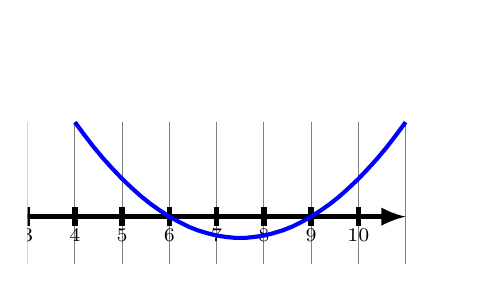
\begin{tikzpicture}[baseline,scale = 0.6]

        \tikzset{ point/.style={ thick, draw, cross out, inner
            sep=0pt, minimum width=5pt, minimum height=5pt, }, } \clip
        (3,-1) rectangle (12,4);
    	
	\draw[color ={black},line width = 2,>=latex,->]
        (-10,0)--(11,0); \draw[color ={black},line width =
        2,>=latex,->] (0,-1)--(0,2); \draw[color ={black},opacity =
        0.5] (1,-1)--(1,2); \draw[color ={black},opacity = 0.5]
        (2,-1)--(2,2); \draw[color ={black},opacity = 0.5]
        (3,-1)--(3,2); \draw[color ={black},opacity = 0.5]
        (4,-1)--(4,2); \draw[color ={black},opacity = 0.5]
        (5,-1)--(5,2); \draw[color ={black},opacity = 0.5]
        (6,-1)--(6,2); \draw[color ={black},opacity = 0.5]
        (7,-1)--(7,2); \draw[color ={black},opacity = 0.5]
        (8,-1)--(8,2); \draw[color ={black},opacity = 0.5]
        (9,-1)--(9,2); \draw[color ={black},opacity = 0.5]
        (10,-1)--(10,2); \draw[color ={black},opacity = 0.5]
        (11,-1)--(11,2); \draw[color ={black},opacity = 0.5]
        (-1,-1)--(-1,2); \draw[color ={black},opacity = 0.5]
        (-2,-1)--(-2,2); \draw[color ={black},opacity = 0.5]
        (-3,-1)--(-3,2); \draw[color ={black},opacity = 0.5]
        (-4,-1)--(-4,2); \draw[color ={black},opacity = 0.5]
        (-5,-1)--(-5,2); \draw[color ={black},opacity = 0.5]
        (-6,-1)--(-6,2); \draw[color ={black},opacity = 0.5]
        (-7,-1)--(-7,2); \draw[color ={black},opacity = 0.5]
        (-8,-1)--(-8,2); \draw[color ={black},opacity = 0.5]
        (-9,-1)--(-9,2); \draw[color ={black},opacity = 0.5]
        (-10,-1)--(-10,2); \draw[color ={black},line width = 2]
        (1,-0.2)--(1,0.2); \draw[color ={black},line width = 2]
        (2,-0.2)--(2,0.2); \draw[color ={black},line width = 2]
        (3,-0.2)--(3,0.2); \draw[color ={black},line width = 2]
        (4,-0.2)--(4,0.2); \draw[color ={black},line width = 2]
        (5,-0.2)--(5,0.2); \draw[color ={black},line width = 2]
        (6,-0.2)--(6,0.2); \draw[color ={black},line width = 2]
        (7,-0.2)--(7,0.2); \draw[color ={black},line width = 2]
        (8,-0.2)--(8,0.2); \draw[color ={black},line width = 2]
        (9,-0.2)--(9,0.2); \draw[color ={black},line width = 2]
        (10,-0.2)--(10,0.2); \draw[color ={black},line width = 2]
        (-1,-0.2)--(-1,0.2); \draw[color ={black},line width = 2]
        (-2,-0.2)--(-2,0.2); \draw[color ={black},line width = 2]
        (-3,-0.2)--(-3,0.2); \draw[color ={black},line width = 2]
        (-4,-0.2)--(-4,0.2); \draw[color ={black},line width = 2]
        (-5,-0.2)--(-5,0.2); \draw[color ={black},line width = 2]
        (-6,-0.2)--(-6,0.2); \draw[color ={black},line width = 2]
        (-7,-0.2)--(-7,0.2); \draw[color ={black},line width = 2]
        (-8,-0.2)--(-8,0.2); \draw[color ={black},line width = 2]
        (-9,-0.2)--(-9,0.2); \draw[color ={black},line width = 2]
        (-0.2,1)--(0.2,1); \draw (1,-0.4) node[anchor = center]
        {\scriptsize \color{black}{$1$}}; \draw (2,-0.4) node[anchor =
        center] {\scriptsize \color{black}{$2$}}; \draw (3,-0.4)
        node[anchor = center] {\scriptsize \color{black}{$3$}}; \draw
        (4,-0.4) node[anchor = center] {\scriptsize
          \color{black}{$4$}}; \draw (5,-0.4) node[anchor = center]
        {\scriptsize \color{black}{$5$}}; \draw (6,-0.4) node[anchor =
        center] {\scriptsize \color{black}{$6$}}; \draw (7,-0.4)
        node[anchor = center] {\scriptsize \color{black}{$7$}}; \draw
        (8,-0.4) node[anchor = center] {\scriptsize
          \color{black}{$8$}}; \draw (9,-0.4) node[anchor = center]
        {\scriptsize \color{black}{$9$}}; \draw (10,-0.4) node[anchor
        = center] {\scriptsize \color{black}{$10$}}; \draw (-1,-0.4)
        node[anchor = center] {\scriptsize \color{black}{$-1$}}; \draw
        (-2,-0.4) node[anchor = center] {\scriptsize
          \color{black}{$-2$}}; \draw (-3,-0.4) node[anchor = center]
        {\scriptsize \color{black}{$-3$}}; \draw (-4,-0.4) node[anchor
        = center] {\scriptsize \color{black}{$-4$}}; \draw (-5,-0.4)
        node[anchor = center] {\scriptsize \color{black}{$-5$}}; \draw
        (-6,-0.4) node[anchor = center] {\scriptsize
          \color{black}{$-6$}}; \draw (-7,-0.4) node[anchor = center]
        {\scriptsize \color{black}{$-7$}}; \draw (-8,-0.4) node[anchor
        = center] {\scriptsize \color{black}{$-8$}}; \draw (-9,-0.4)
        node[anchor = center] {\scriptsize \color{black}{$-9$}}; \draw
        (-0.8,1.1) node[anchor = center] {\footnotesize
          \color{black}{$10$}};
	
	\draw[color={blue},line width = 1.5]
        (4,2)--(4.2,1.73)--(4.4,1.47)--(4.6,1.23)--(4.8,1.01)--(5,0.8)--(5.2,0.61)--(5.4,0.43)--(5.6,0.27)--(5.8,0.13)--(6,0)--(6.2,-0.11)--(6.4,-0.21)--(6.6,-0.29)--(6.8,-0.35)--(7,-0.4)--(7.2,-0.43)--(7.4,-0.45)--(7.6,-0.45)--(7.8,-0.43)--(8,-0.4)--(8.2,-0.35)--(8.4,-0.29)--(8.6,-0.21)--(8.8,-0.11)--(9,0)--(9.2,0.13)--(9.4,0.27)--(9.6,0.43)--(9.8,0.61)--(10,0.8)--(10.2,1.01)--(10.4,1.23)--(10.6,1.47)--(10.8,1.73)--(11,2);

      \end{tikzpicture}\\
    \item Quel est le signe du coefficient dominant de la fonction
      polynomiale $\mathscr{g}$ du second degré représentée ci-dessous
      ?\\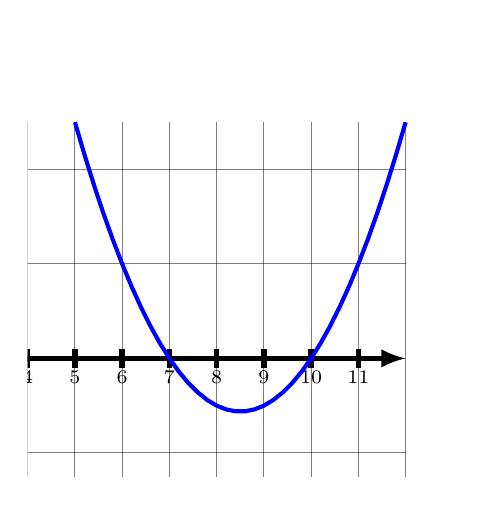
\begin{tikzpicture}[baseline,scale = 0.6]

        \tikzset{ point/.style={ thick, draw, cross out, inner
            sep=0pt, minimum width=5pt, minimum height=5pt, }, } \clip
        (4,-2.5) rectangle (13,7);
    	
	\draw[color ={black},line width = 2,>=latex,->]
        (-10,0)--(12,0); \draw[color ={black},line width =
        2,>=latex,->] (0,-3)--(0,5); \draw[color ={black},opacity =
        0.5] (-10,2)--(12,2); \draw[color ={black},opacity = 0.5]
        (-10,4)--(12,4); \draw[color ={black},opacity = 0.5]
        (-10,-2)--(12,-2); \draw[color ={black},opacity = 0.5]
        (1,-3)--(1,5); \draw[color ={black},opacity = 0.5]
        (2,-3)--(2,5); \draw[color ={black},opacity = 0.5]
        (3,-3)--(3,5); \draw[color ={black},opacity = 0.5]
        (4,-3)--(4,5); \draw[color ={black},opacity = 0.5]
        (5,-3)--(5,5); \draw[color ={black},opacity = 0.5]
        (6,-3)--(6,5); \draw[color ={black},opacity = 0.5]
        (7,-3)--(7,5); \draw[color ={black},opacity = 0.5]
        (8,-3)--(8,5); \draw[color ={black},opacity = 0.5]
        (9,-3)--(9,5); \draw[color ={black},opacity = 0.5]
        (10,-3)--(10,5); \draw[color ={black},opacity = 0.5]
        (11,-3)--(11,5); \draw[color ={black},opacity = 0.5]
        (12,-3)--(12,5); \draw[color ={black},opacity = 0.5]
        (-1,-3)--(-1,5); \draw[color ={black},opacity = 0.5]
        (-2,-3)--(-2,5); \draw[color ={black},opacity = 0.5]
        (-3,-3)--(-3,5); \draw[color ={black},opacity = 0.5]
        (-4,-3)--(-4,5); \draw[color ={black},opacity = 0.5]
        (-5,-3)--(-5,5); \draw[color ={black},opacity = 0.5]
        (-6,-3)--(-6,5); \draw[color ={black},opacity = 0.5]
        (-7,-3)--(-7,5); \draw[color ={black},opacity = 0.5]
        (-8,-3)--(-8,5); \draw[color ={black},opacity = 0.5]
        (-9,-3)--(-9,5); \draw[color ={black},opacity = 0.5]
        (-10,-3)--(-10,5); \draw[color ={black},line width = 2]
        (1,-0.2)--(1,0.2); \draw[color ={black},line width = 2]
        (2,-0.2)--(2,0.2); \draw[color ={black},line width = 2]
        (3,-0.2)--(3,0.2); \draw[color ={black},line width = 2]
        (4,-0.2)--(4,0.2); \draw[color ={black},line width = 2]
        (5,-0.2)--(5,0.2); \draw[color ={black},line width = 2]
        (6,-0.2)--(6,0.2); \draw[color ={black},line width = 2]
        (7,-0.2)--(7,0.2); \draw[color ={black},line width = 2]
        (8,-0.2)--(8,0.2); \draw[color ={black},line width = 2]
        (9,-0.2)--(9,0.2); \draw[color ={black},line width = 2]
        (10,-0.2)--(10,0.2); \draw[color ={black},line width = 2]
        (11,-0.2)--(11,0.2); \draw[color ={black},line width = 2]
        (-1,-0.2)--(-1,0.2); \draw[color ={black},line width = 2]
        (-2,-0.2)--(-2,0.2); \draw[color ={black},line width = 2]
        (-3,-0.2)--(-3,0.2); \draw[color ={black},line width = 2]
        (-4,-0.2)--(-4,0.2); \draw[color ={black},line width = 2]
        (-5,-0.2)--(-5,0.2); \draw[color ={black},line width = 2]
        (-6,-0.2)--(-6,0.2); \draw[color ={black},line width = 2]
        (-7,-0.2)--(-7,0.2); \draw[color ={black},line width = 2]
        (-8,-0.2)--(-8,0.2); \draw[color ={black},line width = 2]
        (-9,-0.2)--(-9,0.2); \draw[color ={black},line width = 2]
        (-0.2,1)--(0.2,1); \draw[color ={black},line width = 2]
        (-0.2,2)--(0.2,2); \draw[color ={black},line width = 2]
        (-0.2,3)--(0.2,3); \draw[color ={black},line width = 2]
        (-0.2,4)--(0.2,4); \draw[color ={black},line width = 2]
        (-0.2,-1)--(0.2,-1); \draw[color ={black},line width = 2]
        (-0.2,-2)--(0.2,-2); \draw (1,-0.4) node[anchor = center]
        {\scriptsize \color{black}{$1$}}; \draw (2,-0.4) node[anchor =
        center] {\scriptsize \color{black}{$2$}}; \draw (3,-0.4)
        node[anchor = center] {\scriptsize \color{black}{$3$}}; \draw
        (4,-0.4) node[anchor = center] {\scriptsize
          \color{black}{$4$}}; \draw (5,-0.4) node[anchor = center]
        {\scriptsize \color{black}{$5$}}; \draw (6,-0.4) node[anchor =
        center] {\scriptsize \color{black}{$6$}}; \draw (7,-0.4)
        node[anchor = center] {\scriptsize \color{black}{$7$}}; \draw
        (8,-0.4) node[anchor = center] {\scriptsize
          \color{black}{$8$}}; \draw (9,-0.4) node[anchor = center]
        {\scriptsize \color{black}{$9$}}; \draw (10,-0.4) node[anchor
        = center] {\scriptsize \color{black}{$10$}}; \draw (11,-0.4)
        node[anchor = center] {\scriptsize \color{black}{$11$}}; \draw
        (-1,-0.4) node[anchor = center] {\scriptsize
          \color{black}{$-1$}}; \draw (-2,-0.4) node[anchor = center]
        {\scriptsize \color{black}{$-2$}}; \draw (-3,-0.4) node[anchor
        = center] {\scriptsize \color{black}{$-3$}}; \draw (-4,-0.4)
        node[anchor = center] {\scriptsize \color{black}{$-4$}}; \draw
        (-5,-0.4) node[anchor = center] {\scriptsize
          \color{black}{$-5$}}; \draw (-6,-0.4) node[anchor = center]
        {\scriptsize \color{black}{$-6$}}; \draw (-7,-0.4) node[anchor
        = center] {\scriptsize \color{black}{$-7$}}; \draw (-8,-0.4)
        node[anchor = center] {\scriptsize \color{black}{$-8$}}; \draw
        (-9,-0.4) node[anchor = center] {\scriptsize
          \color{black}{$-9$}}; \draw (-0.8,1.1) node[anchor = center]
        {\footnotesize \color{black}{$2$}}; \draw (-0.8,2.1)
        node[anchor = center] {\footnotesize \color{black}{$4$}};
        \draw (-0.8,3.1) node[anchor = center] {\footnotesize
          \color{black}{$6$}}; \draw (-0.8,4.1) node[anchor = center]
        {\footnotesize \color{black}{$8$}}; \draw (-0.8,-0.9)
        node[anchor = center] {\footnotesize \color{black}{$-2$}};
        \draw (-0.8,-1.9) node[anchor = center] {\footnotesize
          \color{black}{$-4$}};
	
	\draw[color={blue},line width = 1.5]
        (5,5)--(5.2,4.32)--(5.4,3.68)--(5.6,3.08)--(5.8,2.52)--(6,2)--(6.2,1.52)--(6.4,1.08)--(6.6,0.68)--(6.8,0.32)--(7,0)--(7.2,-0.28)--(7.4,-0.52)--(7.6,-0.72)--(7.8,-0.88)--(8,-1)--(8.2,-1.08)--(8.4,-1.12)--(8.6,-1.12)--(8.8,-1.08)--(9,-1)--(9.2,-0.88)--(9.4,-0.72)--(9.6,-0.52)--(9.8,-0.28)--(10,0)--(10.2,0.32)--(10.4,0.68)--(10.6,1.08)--(10.8,1.52)--(11,2)--(11.2,2.52)--(11.4,3.08)--(11.6,3.68)--(11.8,4.32)--(12,5);

      \end{tikzpicture}\\
    \item Quel est le signe du coefficient dominant de la fonction
      polynomiale $\mathscr{h}$ du second degré représentée ci-dessous
      ?\\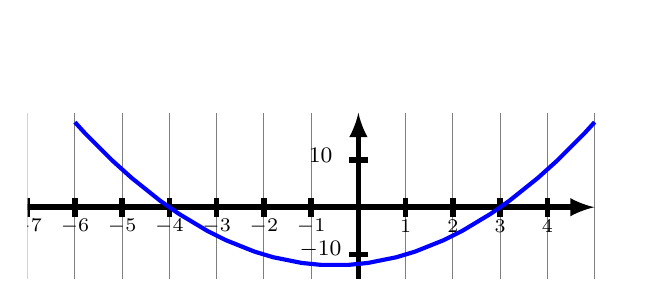
\begin{tikzpicture}[baseline,scale = 0.6]

        \tikzset{ point/.style={ thick, draw, cross out, inner
            sep=0pt, minimum width=5pt, minimum height=5pt, }, } \clip
        (-7,-1.5) rectangle (6,3.8);
    	
	\draw[color ={black},line width = 2,>=latex,->]
        (-10,0)--(5,0); \draw[color ={black},line width =
        2,>=latex,->] (0,-2)--(0,2); \draw[color ={black},opacity =
        0.5] (1,-2)--(1,2); \draw[color ={black},opacity = 0.5]
        (2,-2)--(2,2); \draw[color ={black},opacity = 0.5]
        (3,-2)--(3,2); \draw[color ={black},opacity = 0.5]
        (4,-2)--(4,2); \draw[color ={black},opacity = 0.5]
        (5,-2)--(5,2); \draw[color ={black},opacity = 0.5]
        (-1,-2)--(-1,2); \draw[color ={black},opacity = 0.5]
        (-2,-2)--(-2,2); \draw[color ={black},opacity = 0.5]
        (-3,-2)--(-3,2); \draw[color ={black},opacity = 0.5]
        (-4,-2)--(-4,2); \draw[color ={black},opacity = 0.5]
        (-5,-2)--(-5,2); \draw[color ={black},opacity = 0.5]
        (-6,-2)--(-6,2); \draw[color ={black},opacity = 0.5]
        (-7,-2)--(-7,2); \draw[color ={black},opacity = 0.5]
        (-8,-2)--(-8,2); \draw[color ={black},opacity = 0.5]
        (-9,-2)--(-9,2); \draw[color ={black},opacity = 0.5]
        (-10,-2)--(-10,2); \draw[color ={black},line width = 2]
        (1,-0.2)--(1,0.2); \draw[color ={black},line width = 2]
        (2,-0.2)--(2,0.2); \draw[color ={black},line width = 2]
        (3,-0.2)--(3,0.2); \draw[color ={black},line width = 2]
        (4,-0.2)--(4,0.2); \draw[color ={black},line width = 2]
        (-1,-0.2)--(-1,0.2); \draw[color ={black},line width = 2]
        (-2,-0.2)--(-2,0.2); \draw[color ={black},line width = 2]
        (-3,-0.2)--(-3,0.2); \draw[color ={black},line width = 2]
        (-4,-0.2)--(-4,0.2); \draw[color ={black},line width = 2]
        (-5,-0.2)--(-5,0.2); \draw[color ={black},line width = 2]
        (-6,-0.2)--(-6,0.2); \draw[color ={black},line width = 2]
        (-7,-0.2)--(-7,0.2); \draw[color ={black},line width = 2]
        (-8,-0.2)--(-8,0.2); \draw[color ={black},line width = 2]
        (-9,-0.2)--(-9,0.2); \draw[color ={black},line width = 2]
        (-0.2,1)--(0.2,1); \draw[color ={black},line width = 2]
        (-0.2,-1)--(0.2,-1); \draw (1,-0.4) node[anchor = center]
        {\scriptsize \color{black}{$1$}}; \draw (2,-0.4) node[anchor =
        center] {\scriptsize \color{black}{$2$}}; \draw (3,-0.4)
        node[anchor = center] {\scriptsize \color{black}{$3$}}; \draw
        (4,-0.4) node[anchor = center] {\scriptsize
          \color{black}{$4$}}; \draw (-1,-0.4) node[anchor = center]
        {\scriptsize \color{black}{$-1$}}; \draw (-2,-0.4) node[anchor
        = center] {\scriptsize \color{black}{$-2$}}; \draw (-3,-0.4)
        node[anchor = center] {\scriptsize \color{black}{$-3$}}; \draw
        (-4,-0.4) node[anchor = center] {\scriptsize
          \color{black}{$-4$}}; \draw (-5,-0.4) node[anchor = center]
        {\scriptsize \color{black}{$-5$}}; \draw (-6,-0.4) node[anchor
        = center] {\scriptsize \color{black}{$-6$}}; \draw (-7,-0.4)
        node[anchor = center] {\scriptsize \color{black}{$-7$}}; \draw
        (-8,-0.4) node[anchor = center] {\scriptsize
          \color{black}{$-8$}}; \draw (-9,-0.4) node[anchor = center]
        {\scriptsize \color{black}{$-9$}}; \draw (-0.8,1.1)
        node[anchor = center] {\footnotesize \color{black}{$10$}};
        \draw (-0.8,-0.9) node[anchor = center] {\footnotesize
          \color{black}{$-10$}};
	
	\draw[color={blue},line width = 1.5]
        (-6,1.8)--(-5.8,1.58)--(-5.6,1.38)--(-5.4,1.18)--(-5.2,0.98)--(-5,0.8)--(-4.8,0.62)--(-4.6,0.46)--(-4.4,0.3)--(-4.2,0.14)--(-4,0)--(-3.8,-0.14)--(-3.6,-0.26)--(-3.4,-0.38)--(-3.2,-0.5)--(-3,-0.6)--(-2.8,-0.7)--(-2.6,-0.78)--(-2.4,-0.86)--(-2.2,-0.94)--(-2,-1)--(-1.8,-1.06)--(-1.6,-1.1)--(-1.4,-1.14)--(-1.2,-1.18)--(-1,-1.2)--(-0.8,-1.22)--(-0.6,-1.22)--(-0.4,-1.22)--(-0.2,-1.22)--(0,-1.2)--(0.2,-1.18)--(0.4,-1.14)--(0.6,-1.1)--(0.8,-1.06)--(1,-1)--(1.2,-0.94)--(1.4,-0.86)--(1.6,-0.78)--(1.8,-0.7)--(2,-0.6)--(2.2,-0.5)--(2.4,-0.38)--(2.6,-0.26)--(2.8,-0.14)--(3,0)--(3.2,0.14)--(3.4,0.3)--(3.6,0.46)--(3.8,0.62)--(4,0.8)--(4.2,0.98)--(4.4,1.18)--(4.6,1.38)--(4.8,1.58)--(5,1.8);

      \end{tikzpicture}\\
    \item Quel est le signe du coefficient dominant de la fonction
      polynomiale $\mathscr{i}$ du second degré représentée ci-dessous
      ?\\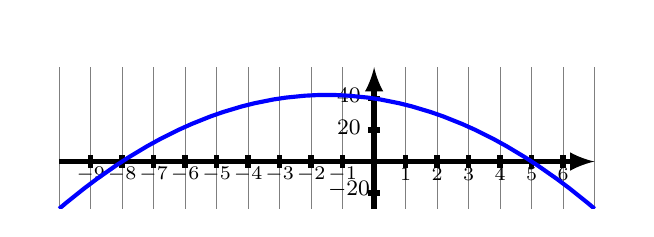
\begin{tikzpicture}[baseline,scale = 0.4]

        \tikzset{ point/.style={ thick, draw, cross out, inner
            sep=0pt, minimum width=5pt, minimum height=5pt, }, } \clip
        (-11,-1.5) rectangle (8,4.25);
    	
	\draw[color ={black},line width = 2,>=latex,->]
        (-10,0)--(7,0); \draw[color ={black},line width =
        2,>=latex,->] (0,-2)--(0,3); \draw[color ={black},opacity =
        0.5] (1,-2)--(1,3); \draw[color ={black},opacity = 0.5]
        (2,-2)--(2,3); \draw[color ={black},opacity = 0.5]
        (3,-2)--(3,3); \draw[color ={black},opacity = 0.5]
        (4,-2)--(4,3); \draw[color ={black},opacity = 0.5]
        (5,-2)--(5,3); \draw[color ={black},opacity = 0.5]
        (6,-2)--(6,3); \draw[color ={black},opacity = 0.5]
        (7,-2)--(7,3); \draw[color ={black},opacity = 0.5]
        (-1,-2)--(-1,3); \draw[color ={black},opacity = 0.5]
        (-2,-2)--(-2,3); \draw[color ={black},opacity = 0.5]
        (-3,-2)--(-3,3); \draw[color ={black},opacity = 0.5]
        (-4,-2)--(-4,3); \draw[color ={black},opacity = 0.5]
        (-5,-2)--(-5,3); \draw[color ={black},opacity = 0.5]
        (-6,-2)--(-6,3); \draw[color ={black},opacity = 0.5]
        (-7,-2)--(-7,3); \draw[color ={black},opacity = 0.5]
        (-8,-2)--(-8,3); \draw[color ={black},opacity = 0.5]
        (-9,-2)--(-9,3); \draw[color ={black},opacity = 0.5]
        (-10,-2)--(-10,3); \draw[color ={black},line width = 2]
        (1,-0.2)--(1,0.2); \draw[color ={black},line width = 2]
        (2,-0.2)--(2,0.2); \draw[color ={black},line width = 2]
        (3,-0.2)--(3,0.2); \draw[color ={black},line width = 2]
        (4,-0.2)--(4,0.2); \draw[color ={black},line width = 2]
        (5,-0.2)--(5,0.2); \draw[color ={black},line width = 2]
        (6,-0.2)--(6,0.2); \draw[color ={black},line width = 2]
        (-1,-0.2)--(-1,0.2); \draw[color ={black},line width = 2]
        (-2,-0.2)--(-2,0.2); \draw[color ={black},line width = 2]
        (-3,-0.2)--(-3,0.2); \draw[color ={black},line width = 2]
        (-4,-0.2)--(-4,0.2); \draw[color ={black},line width = 2]
        (-5,-0.2)--(-5,0.2); \draw[color ={black},line width = 2]
        (-6,-0.2)--(-6,0.2); \draw[color ={black},line width = 2]
        (-7,-0.2)--(-7,0.2); \draw[color ={black},line width = 2]
        (-8,-0.2)--(-8,0.2); \draw[color ={black},line width = 2]
        (-9,-0.2)--(-9,0.2); \draw[color ={black},line width = 2]
        (-0.2,1)--(0.2,1); \draw[color ={black},line width = 2]
        (-0.2,2)--(0.2,2); \draw[color ={black},line width = 2]
        (-0.2,-1)--(0.2,-1); \draw (1,-0.4) node[anchor = center]
        {\scriptsize \color{black}{$1$}}; \draw (2,-0.4) node[anchor =
        center] {\scriptsize \color{black}{$2$}}; \draw (3,-0.4)
        node[anchor = center] {\scriptsize \color{black}{$3$}}; \draw
        (4,-0.4) node[anchor = center] {\scriptsize
          \color{black}{$4$}}; \draw (5,-0.4) node[anchor = center]
        {\scriptsize \color{black}{$5$}}; \draw (6,-0.4) node[anchor =
        center] {\scriptsize \color{black}{$6$}}; \draw (-1,-0.4)
        node[anchor = center] {\scriptsize \color{black}{$-1$}}; \draw
        (-2,-0.4) node[anchor = center] {\scriptsize
          \color{black}{$-2$}}; \draw (-3,-0.4) node[anchor = center]
        {\scriptsize \color{black}{$-3$}}; \draw (-4,-0.4) node[anchor
        = center] {\scriptsize \color{black}{$-4$}}; \draw (-5,-0.4)
        node[anchor = center] {\scriptsize \color{black}{$-5$}}; \draw
        (-6,-0.4) node[anchor = center] {\scriptsize
          \color{black}{$-6$}}; \draw (-7,-0.4) node[anchor = center]
        {\scriptsize \color{black}{$-7$}}; \draw (-8,-0.4) node[anchor
        = center] {\scriptsize \color{black}{$-8$}}; \draw (-9,-0.4)
        node[anchor = center] {\scriptsize \color{black}{$-9$}}; \draw
        (-0.8,1.1) node[anchor = center] {\footnotesize
          \color{black}{$20$}}; \draw (-0.8,2.1) node[anchor = center]
        {\footnotesize \color{black}{$40$}}; \draw (-0.8,-0.9)
        node[anchor = center] {\footnotesize \color{black}{$-20$}};
	
	\draw[color={blue},line width = 1.5]
        (-10,-1.5)--(-9.8,-1.33)--(-9.6,-1.17)--(-9.4,-1.01)--(-9.2,-0.85)--(-9,-0.7)--(-8.8,-0.55)--(-8.6,-0.41)--(-8.4,-0.27)--(-8.2,-0.13)--(-8,0)--(-7.8,0.13)--(-7.6,0.25)--(-7.4,0.37)--(-7.2,0.49)--(-7,0.6)--(-6.8,0.71)--(-6.6,0.81)--(-6.4,0.91)--(-6.2,1.01)--(-6,1.1)--(-5.8,1.19)--(-5.6,1.27)--(-5.4,1.35)--(-5.2,1.43)--(-5,1.5)--(-4.8,1.57)--(-4.6,1.63)--(-4.4,1.69)--(-4.2,1.75)--(-4,1.8)--(-3.8,1.85)--(-3.6,1.89)--(-3.4,1.93)--(-3.2,1.97)--(-3,2)--(-2.8,2.03)--(-2.6,2.05)--(-2.4,2.07)--(-2.2,2.09)--(-2,2.1)--(-1.8,2.11)--(-1.6,2.11)--(-1.4,2.11)--(-1.2,2.11)--(-1,2.1)--(-0.8,2.09)--(-0.6,2.07)--(-0.4,2.05)--(-0.2,2.03)--(0,2)--(0.2,1.97)--(0.4,1.93)--(0.6,1.89)--(0.8,1.85)--(1,1.8)--(1.2,1.75)--(1.4,1.69)--(1.6,1.63)--(1.8,1.57)--(2,1.5)--(2.2,1.43)--(2.4,1.35)--(2.6,1.27)--(2.8,1.19)--(3,1.1)--(3.2,1.01)--(3.4,0.91)--(3.6,0.81)--(3.8,0.71)--(4,0.6)--(4.2,0.49)--(4.4,0.37)--(4.6,0.25)--(4.8,0.13)--(5,0)--(5.2,-0.13)--(5.4,-0.27)--(5.6,-0.41)--(5.8,-0.55)--(6,-0.7)--(6.2,-0.85)--(6.4,-1.01)--(6.6,-1.17)--(6.8,-1.33)--(7,-1.5);

      \end{tikzpicture}
\item Quel est le signe du coefficient dominant de la fonction polynomiale $\mathscr{f}$ du second degré représentée ci-dessous ?\\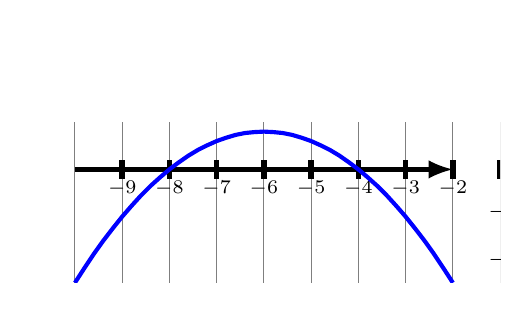
\begin{tikzpicture}[baseline,scale = 0.6]

    \tikzset{
      point/.style={
        thick,
        draw,
        cross out,
        inner sep=0pt,
        minimum width=5pt,
        minimum height=5pt,
      },
    }
    \clip (-11,-2.4) rectangle (-1,3);
    	
	\draw[color ={black},line width = 2,>=latex,->] (-10,0)--(-2,0);
	\draw[color ={black},line width = 2,>=latex,->] (0,-3)--(0,1);
	\draw[color ={black},opacity = 0.5] (-1,-3)--(-1,1);
	\draw[color ={black},opacity = 0.5] (-2,-3)--(-2,1);
	\draw[color ={black},opacity = 0.5] (-3,-3)--(-3,1);
	\draw[color ={black},opacity = 0.5] (-4,-3)--(-4,1);
	\draw[color ={black},opacity = 0.5] (-5,-3)--(-5,1);
	\draw[color ={black},opacity = 0.5] (-6,-3)--(-6,1);
	\draw[color ={black},opacity = 0.5] (-7,-3)--(-7,1);
	\draw[color ={black},opacity = 0.5] (-8,-3)--(-8,1);
	\draw[color ={black},opacity = 0.5] (-9,-3)--(-9,1);
	\draw[color ={black},opacity = 0.5] (-10,-3)--(-10,1);
	\draw[color ={black},line width = 2] (-1,-0.2)--(-1,0.2);
	\draw[color ={black},line width = 2] (-2,-0.2)--(-2,0.2);
	\draw[color ={black},line width = 2] (-3,-0.2)--(-3,0.2);
	\draw[color ={black},line width = 2] (-4,-0.2)--(-4,0.2);
	\draw[color ={black},line width = 2] (-5,-0.2)--(-5,0.2);
	\draw[color ={black},line width = 2] (-6,-0.2)--(-6,0.2);
	\draw[color ={black},line width = 2] (-7,-0.2)--(-7,0.2);
	\draw[color ={black},line width = 2] (-8,-0.2)--(-8,0.2);
	\draw[color ={black},line width = 2] (-9,-0.2)--(-9,0.2);
	\draw[color ={black},line width = 2] (-0.2,-1)--(0.2,-1);
	\draw[color ={black},line width = 2] (-0.2,-2)--(0.2,-2);
	\draw (-2,-0.4) node[anchor = center] {\scriptsize \color{black}{$-2$}};
	\draw (-3,-0.4) node[anchor = center] {\scriptsize \color{black}{$-3$}};
	\draw (-4,-0.4) node[anchor = center] {\scriptsize \color{black}{$-4$}};
	\draw (-5,-0.4) node[anchor = center] {\scriptsize \color{black}{$-5$}};
	\draw (-6,-0.4) node[anchor = center] {\scriptsize \color{black}{$-6$}};
	\draw (-7,-0.4) node[anchor = center] {\scriptsize \color{black}{$-7$}};
	\draw (-8,-0.4) node[anchor = center] {\scriptsize \color{black}{$-8$}};
	\draw (-9,-0.4) node[anchor = center] {\scriptsize \color{black}{$-9$}};
	\draw (-0.8,-0.9) node[anchor = center] {\footnotesize \color{black}{$-10$}};
	\draw (-0.8,-1.9) node[anchor = center] {\footnotesize \color{black}{$-20$}};
	
	\draw[color={blue},line width = 1.5] (-10,-2.4)--(-9.8,-2.09)--(-9.6,-1.79)--(-9.4,-1.51)--(-9.2,-1.25)--(-9,-1)--(-8.8,-0.77)--(-8.6,-0.55)--(-8.4,-0.35)--(-8.2,-0.17)--(-8,0)--(-7.8,0.15)--(-7.6,0.29)--(-7.4,0.41)--(-7.2,0.51)--(-7,0.6)--(-6.8,0.67)--(-6.6,0.73)--(-6.4,0.77)--(-6.2,0.79)--(-6,0.8)--(-5.8,0.79)--(-5.6,0.77)--(-5.4,0.73)--(-5.2,0.67)--(-5,0.6)--(-4.8,0.51)--(-4.6,0.41)--(-4.4,0.29)--(-4.2,0.15)--(-4,0)--(-3.8,-0.17)--(-3.6,-0.35)--(-3.4,-0.55)--(-3.2,-0.77)--(-3,-1)--(-2.8,-1.25)--(-2.6,-1.51)--(-2.4,-1.79)--(-2.2,-2.09)--(-2,-2.4);

\end{tikzpicture}\\
	\item Quel est le signe du coefficient dominant de la fonction polynomiale $\mathscr{g}$ du second degré représentée ci-dessous ?\\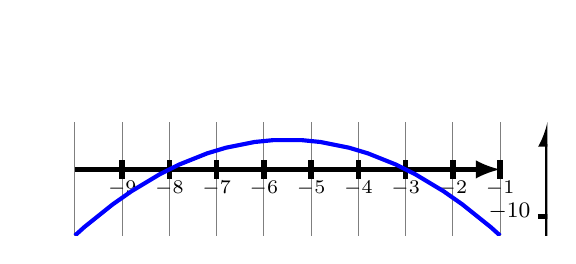
\begin{tikzpicture}[baseline,scale = 0.6]

    \tikzset{
      point/.style={
        thick,
        draw,
        cross out,
        inner sep=0pt,
        minimum width=5pt,
        minimum height=5pt,
      },
    }
    \clip (-11,-1.4) rectangle (0,3);
    	
	\draw[color ={black},line width = 2,>=latex,->] (-10,0)--(-1,0);
	\draw[color ={black},line width = 2,>=latex,->] (0,-2)--(0,1);
	\draw[color ={black},opacity = 0.5] (-1,-2)--(-1,1);
	\draw[color ={black},opacity = 0.5] (-2,-2)--(-2,1);
	\draw[color ={black},opacity = 0.5] (-3,-2)--(-3,1);
	\draw[color ={black},opacity = 0.5] (-4,-2)--(-4,1);
	\draw[color ={black},opacity = 0.5] (-5,-2)--(-5,1);
	\draw[color ={black},opacity = 0.5] (-6,-2)--(-6,1);
	\draw[color ={black},opacity = 0.5] (-7,-2)--(-7,1);
	\draw[color ={black},opacity = 0.5] (-8,-2)--(-8,1);
	\draw[color ={black},opacity = 0.5] (-9,-2)--(-9,1);
	\draw[color ={black},opacity = 0.5] (-10,-2)--(-10,1);
	\draw[color ={black},line width = 2] (-1,-0.2)--(-1,0.2);
	\draw[color ={black},line width = 2] (-2,-0.2)--(-2,0.2);
	\draw[color ={black},line width = 2] (-3,-0.2)--(-3,0.2);
	\draw[color ={black},line width = 2] (-4,-0.2)--(-4,0.2);
	\draw[color ={black},line width = 2] (-5,-0.2)--(-5,0.2);
	\draw[color ={black},line width = 2] (-6,-0.2)--(-6,0.2);
	\draw[color ={black},line width = 2] (-7,-0.2)--(-7,0.2);
	\draw[color ={black},line width = 2] (-8,-0.2)--(-8,0.2);
	\draw[color ={black},line width = 2] (-9,-0.2)--(-9,0.2);
	\draw[color ={black},line width = 2] (-0.2,-1)--(0.2,-1);
	\draw (-1,-0.4) node[anchor = center] {\scriptsize \color{black}{$-1$}};
	\draw (-2,-0.4) node[anchor = center] {\scriptsize \color{black}{$-2$}};
	\draw (-3,-0.4) node[anchor = center] {\scriptsize \color{black}{$-3$}};
	\draw (-4,-0.4) node[anchor = center] {\scriptsize \color{black}{$-4$}};
	\draw (-5,-0.4) node[anchor = center] {\scriptsize \color{black}{$-5$}};
	\draw (-6,-0.4) node[anchor = center] {\scriptsize \color{black}{$-6$}};
	\draw (-7,-0.4) node[anchor = center] {\scriptsize \color{black}{$-7$}};
	\draw (-8,-0.4) node[anchor = center] {\scriptsize \color{black}{$-8$}};
	\draw (-9,-0.4) node[anchor = center] {\scriptsize \color{black}{$-9$}};
	\draw (-0.8,-0.9) node[anchor = center] {\footnotesize \color{black}{$-10$}};
	
	\draw[color={blue},line width = 1.5] (-10,-1.4)--(-9.8,-1.22)--(-9.6,-1.06)--(-9.4,-0.9)--(-9.2,-0.74)--(-9,-0.6)--(-8.8,-0.46)--(-8.6,-0.34)--(-8.4,-0.22)--(-8.2,-0.1)--(-8,0)--(-7.8,0.1)--(-7.6,0.18)--(-7.4,0.26)--(-7.2,0.34)--(-7,0.4)--(-6.8,0.46)--(-6.6,0.5)--(-6.4,0.54)--(-6.2,0.58)--(-6,0.6)--(-5.8,0.62)--(-5.6,0.62)--(-5.4,0.62)--(-5.2,0.62)--(-5,0.6)--(-4.8,0.58)--(-4.6,0.54)--(-4.4,0.5)--(-4.2,0.46)--(-4,0.4)--(-3.8,0.34)--(-3.6,0.26)--(-3.4,0.18)--(-3.2,0.1)--(-3,0)--(-2.8,-0.1)--(-2.6,-0.22)--(-2.4,-0.34)--(-2.2,-0.46)--(-2,-0.6)--(-1.8,-0.74)--(-1.6,-0.9)--(-1.4,-1.06)--(-1.2,-1.22)--(-1,-1.4);

\end{tikzpicture}\\      
    \end{enumerate}
  \end{multicols}
\end{exercice}

\end{document}




%%% Local Variables:
%%% mode: LaTeX
%%% TeX-master: t
%%% End:
